%%%%%%%%%% *** The Title %%%%%%%%%%
\title[]{지표와 대기의 가열\\ \small{제2장}}

\begin{frame}[plain] %title page
	\titlepage
\end{frame}


\begin{frame}[plain] %cc page
	\ccpage
\end{frame}


\section{지구와 태양의 관계}


\begin{frame}[t]{계절의 변화}
	\begin{tabular}{ll}
		\begin{minipage}[t]{0.90\textwidth}
			\begin{figure}{}
				\includegraphics[trim=35 40 30 505, clip, page=61, width=\textwidth]{\bookfile}\\
			\end{figure}
			\begin{itemize}
				\item 4계절의 아름다움 
				\item 계절을 이해하기 위해서는 지구와 태양의 관계를 이해해야 한다.
			\end{itemize}			
		\end{minipage}
	\end{tabular}
\end{frame}



\begin{frame}[t]{지구의 운동: 공전}
	\begin{tabular}{ll}
		\begin{minipage}[t]{0.65\textwidth}
			\begin{figure}{}
				\includegraphics[trim=65 525 255 60, 
				clip, page=62, width=\textwidth]{\bookfile}\\
			\end{figure}
			\scriptsize
			\begin{itemize}
				\item 지구 공전궤도의 이심률: $0.0167$
				\item 지구 궤도 장반경 : $1.495978875 \times 10^{11} \rm{~m}$
			\end{itemize}
			
		\end{minipage} 
		&
		\begin{minipage}[t]{0.3\textwidth}
			\questionset {근일점과 원일점에서의 태양까지의 거리 비는 얼마인가?}
			\solutionset{$ \dfrac{a(1+e)}{a(1-e)}$ = 1.034	\newline}
			
			\questionset {북반구의 계절이 겨울일 때 지구와 태양 사이 거리는 어떠한가?}
			\solutionset{지구는 공전궤도 이심률이 작아서 근일점과 원일점의 거리차가 크지는 않지만, 1월 3일 경에 근일점 근처, 7월 4일 경에 원일점에 위치하므로, 북반구 계절이 겨울일때 태양과 지구 사이의 거리는 좀 더 가깝다.}
		\end{minipage}
	\end{tabular}
\end{frame}




\begin{frame}[t]{태양의 고도 변화}
	\begin{tabular}{ll}
		\begin{minipage}[t]{0.95\textwidth}
			\begin{figure}{}
				\includegraphics[trim=45 37 15 525, clip, page=62, width=\textwidth]{\bookfile}
			\end{figure}
			\begin{itemize}
				\item 태양에 수직일 때의 태양의 복사 강도를 $I_{0}$, 태양의 고도각이 $\alpha$일 때의 태양의 복사 강도를 $I_{\alpha}$라 하면 $I_{\alpha} = I_0 \sin{\alpha} $가 된다.
			\end{itemize}
		\end{minipage} 
		&
		\begin{minipage}[t]{0.03\textwidth}
			
		\end{minipage}
	\end{tabular}
\end{frame}




\begin{frame}[t]{위도에 따른 변화}
	\begin{tabular}{ll}
		\begin{minipage}[t]{0.50\textwidth}
			\begin{figure}
				\includegraphics[trim=35 440 365 55, clip, page=63, width=\textwidth]{\bookfile}
			\end{figure}
		\end{minipage}
		&
		\begin{minipage}[t]{0.45\textwidth}
			\begin{block}{고위도로 갈수록}
				\begin{itemize}
					\item 태양광선이 대기를 통과하는 두께가 두꺼워지고
					\item 태양의 고도가 낮아져서 
					\item 따라서 단위 면적 당 도달하는 복사에너지가 작아진다.
				\end{itemize}
			\end{block}
		\end{minipage}
	\end{tabular} 
\end{frame}



\begin{frame}[t]{자전축의 경사}
	\begin{tabular}{ll}
		\begin{minipage}[t]{0.9\textwidth}
			\begin{figure}{}
				\includegraphics[trim=40 45 60 465, clip, page=63, width=0.9\textwidth]{\bookfile}
			\end{figure}
		\end{minipage}
		&
		\begin{minipage}[t]{0.05\textwidth}
		\end{minipage}
	\end{tabular}
	\begin{itemize}\scriptsize
		\item 지구의 공전면과 지구의 자전축이 수직이 아니고, 수직면에서 $23.5 \rm{^\circ}$ 기울어짐
		\item 지구의 자전축이 하지에는 북반구가 태양쪽으로 $23.5 \rm{^\circ}$ 기울어진 위치이며, 동지에는 태양의 반대편으로 $23.5 \rm{^\circ}$ 기울어짐.
		\item 춘분과 추분에는 태양이 적도지방을 수직으로 비치게 된다.
	\end{itemize}
\end{frame}




\begin{frame}[t]{태양의 남중 고도}
	\begin{tabular}{ll}
		\begin{minipage}[t]{0.40\textwidth}
			\begin{figure}
				\includegraphics[trim=160 475 245 110, clip, page=65, width=\textwidth]{\bookfile}
			\end{figure}
		\end{minipage}
		&
		\begin{minipage}[t]{0.55\textwidth}
			\questionset{태양의 남중고도는 어떻게 구할수 있는가?}
			\solutionset{$h = 90{^\circ} - \varphi + \delta$ \\
				(남중고도) = ($90^{^\circ}$ - 위도 + 적위)}
		\end{minipage}
	\end{tabular} 
\end{frame}


\begin{frame}[t]{낮의 길이}
	\begin{tabular}{ll}
		\begin{minipage}[t]{0.55\textwidth}
			\centering
			\begin{figure}{}
			\includegraphics[trim=70 375 130 70, clip, page=64, width=\textwidth]{\bookfile}\\
			\end{figure}
		\end{minipage}
		&
		\begin{minipage}[t]{0.40\textwidth}
			\begin{itemize} \scriptsize 
				\item 북반구의 경우, 
				하지 때는 낮의 길이(밝은 부분)가 밤의 길이(어두운 부분)보다 길고, 
				\item 동지 때는 밤의 길이가 낮의 길이보다 길다.  
				\item 단, 위도에 따라 낮과 밤의 길이 차이는 다르다.
			\end{itemize}
				\questionset{계절별 온도 변화의 원인 두가지를 고르면?}
				\solutionset{1. 계절에 따른 태양의 고도(태양각) 변화\\
				2. 계절에 따른 낮의 길이의 변화}
		\end{minipage}
	\end{tabular}
\end{frame}



\begin{frame}[t]{위도별 낮의 길이}
	\begin{tabular}{ll}
		\begin{minipage}[t]{.45\textwidth}
			\centering
			\begin{figure}{}
				\includegraphics[trim=40 50 370 550, clip, page=65, width=\textwidth]{\bookfile}
			\end{figure}
		\end{minipage}
		&
		\begin{minipage}[t]{0.5\textwidth}
			\questionset{적도 지방의 낮의 길이는 어떠한가?}
			\solutionset{적도에서는 연중, 낮과 밤의 길이가 같다.\newline}
			
			\questionset{고위도 지방의 낮의 길이는 어떠한가?}
			\solutionset{위도 $70{^\circ}$ 이상인 지역에서는 해가 지지 않는 날이 있을 수 있으며, 북극, 남극에서는 6개월 동안 해가 지지 않는다. \newline}	
			
			\questionset{춘분, 추분날 낮과 밤의 길이는 어떠한가?}
			\solutionset{극을 제외한 지구 상 어느 곳에서나 낮과 밤의 길이가 같다. }
		\end{minipage}
	\end{tabular}	
\end{frame}







\begin{frame}[t]{하루 동안 태양의 경로}
	\begin{tabular}{ll}
		\begin{minipage}[t]{.6\textwidth}
			\begin{figure}{}
				\includegraphics[trim=70 40 162 440, 
				clip, page=66, width=\textwidth]{\bookfile} 
			\end{figure}
		\end{minipage}
		&
		\begin{minipage}[t]{.35\textwidth}
			\questionset{위도를 $37.5\rm{^\circ}N$ 지점에서의 하지날과 동지날 낮의 길이를 각각 구하시오. (단, 하지날 태양의 적위는 $+23.5{^\circ}$이다.)}
			\solutionset{적위 $\delta$ , 고도 $h$, 위도 $\varphi$ , 시간각 $H$ 라고 두면, \\
				$\sin h=\cos H \cos \varphi \cos \delta+\sin \varphi \sin \delta$를 이용해 보자.
				해가 뜰 때의 고도 $h$는 $0{^\circ}$ 이므로 \\
				$\cos H=-\tan \delta \tan \varphi$\\
				1) 하지날의 시간각 $H = 109.4901{^\circ} = 7^h ~17^m~ 58^s$이므로, 낮의 길이는 시간각의 두 배로 $14^h ~35^m ~56^s$ 이다.\\
				2) 동지날의 시간각 $H = 70.5099{^\circ} = 4^h ~42^m ~2^s$ 이므로, 낮의 길이는 시간각의 두 배로 $9^h ~24^m ~4^s$ 이다.}
		\end{minipage}
	\end{tabular}
\end{frame}





\begin{frame}[t]{낮의 길이}
	\begin{tabular}{ll}
		\begin{minipage}[t]{.65\textwidth}
			\begin{figure}{}
				
				\tikzset{every picture/.style={line width=0.75pt}} %set default line width to 0.75pt        
				
				\begin{tikzpicture}[x=0.75pt,y=0.75pt,yscale=-1,xscale=1]
					%uncomment if require: \path (0,181); %set diagram left start at 0, and has height of 181
					
					%Shape: Circle [id:dp9794768611549483] 
					\draw  [line width=1.5]  (81,88.5) .. controls (81,50.12) and (112.12,19) .. (150.5,19) .. controls (188.88,19) and (220,50.12) .. (220,88.5) .. controls (220,126.88) and (188.88,158) .. (150.5,158) .. controls (112.12,158) and (81,126.88) .. (81,88.5) -- cycle ;
					%Straight Lines [id:da7004238529168441] 
					\draw    (150,170) -- (150,10) ;
					%Straight Lines [id:da7067154493558592] 
					\draw    (70,90) -- (228.67,90) ;
					%Straight Lines [id:da06857530791005506] 
					\draw    (70.67,121.17) -- (229.67,61.17) ;
					%Straight Lines [id:da6872867799837892] 
					\draw [color={rgb, 255:red, 0; green, 0; blue, 255 }  ,draw opacity=1 ][line width=1.5]    (110,170) -- (191,10.5) ;
					%Straight Lines [id:da020726952306879598] 
					\draw [color={rgb, 255:red, 255; green, 0; blue, 0 }  ,draw opacity=1 ][line width=1.5]    (87.92,59.08) -- (210.75,120.92) ;
					%Shape: Circle [id:dp7840156767396058] 
					\draw  [line width=1.5]  (260,89.5) .. controls (260,56.64) and (286.64,30) .. (319.5,30) .. controls (352.36,30) and (379,56.64) .. (379,89.5) .. controls (379,122.36) and (352.36,149) .. (319.5,149) .. controls (286.64,149) and (260,122.36) .. (260,89.5) -- cycle ;
					%Straight Lines [id:da13899044112002357] 
					\draw    (319.5,168.5) -- (319.5,10.5) ;
					%Straight Lines [id:da8417096202711019] 
					\draw [color={rgb, 255:red, 0; green, 255; blue, 0 }  ,draw opacity=1 ][line width=1.5]    (319.5,89.5) -- (290,39) ;
					%Straight Lines [id:da49526579548449123] 
					\draw [color={rgb, 255:red, 0; green, 255; blue, 0 }  ,draw opacity=1 ][line width=1.5]    (290,140) -- (319.5,89.5) ;
					%Straight Lines [id:da6412141101483668] 
					\draw    (290,140) -- (290,39) ;
					%Straight Lines [id:da41117475249815105] 
					\draw [color={rgb, 255:red, 139; green, 87; blue, 42 }  ,draw opacity=1 ][line width=1.5]    (290,89.5) -- (319.5,89.5) ;
					%Straight Lines [id:da3534831220634276] 
					\draw [color={rgb, 255:red, 0; green, 255; blue, 0 }  ,draw opacity=1 ][line width=1.5]    (215.67,66.17) -- (174.67,43.67) ;
					%Straight Lines [id:da3310423092199495] 
					\draw [color={rgb, 255:red, 74; green, 144; blue, 226 }  ,draw opacity=1 ]   (267.67,39.17) -- (300.29,58.96) ;
					\draw [shift={(302,60)}, rotate = 211.25] [fill={rgb, 255:red, 74; green, 144; blue, 226 }  ,fill opacity=1 ][line width=0.08]  [draw opacity=0] (12,-3) -- (0,0) -- (12,3) -- cycle    ;
					%Straight Lines [id:da12755818672809105] 
					\draw [color={rgb, 255:red, 74; green, 144; blue, 226 }  ,draw opacity=1 ]   (234.67,40.17) -- (201.49,55.34) ;
					\draw [shift={(199.67,56.17)}, rotate = 335.43] [fill={rgb, 255:red, 74; green, 144; blue, 226 }  ,fill opacity=1 ][line width=0.08]  [draw opacity=0] (12,-3) -- (0,0) -- (12,3) -- cycle    ;
					%Straight Lines [id:da3129894649743603] 
					\draw [color={rgb, 255:red, 74; green, 144; blue, 226 }  ,draw opacity=1 ]   (95.67,29.17) -- (164.15,57.24) ;
					\draw [shift={(166,58)}, rotate = 202.29] [fill={rgb, 255:red, 74; green, 144; blue, 226 }  ,fill opacity=1 ][line width=0.08]  [draw opacity=0] (12,-3) -- (0,0) -- (12,3) -- cycle    ;
					%Straight Lines [id:da980416960713657] 
					\draw [color={rgb, 255:red, 139; green, 87; blue, 42 }  ,draw opacity=1 ][line width=1.5]    (150.67,31.17) -- (174.67,43.67) ;
					%Straight Lines [id:da589694860813891] 
					\draw [color={rgb, 255:red, 74; green, 144; blue, 226 }  ,draw opacity=1 ]   (255.67,152.17) -- (303.52,91.07) ;
					\draw [shift={(304.75,89.5)}, rotate = 488.07] [fill={rgb, 255:red, 74; green, 144; blue, 226 }  ,fill opacity=1 ][line width=0.08]  [draw opacity=0] (12,-3) -- (0,0) -- (12,3) -- cycle    ;
					%Straight Lines [id:da14235935968093516] 
					\draw [color={rgb, 255:red, 74; green, 144; blue, 226 }  ,draw opacity=1 ]   (240.92,152.17) -- (163.79,39.07) ;
					\draw [shift={(162.67,37.42)}, rotate = 415.71000000000004] [fill={rgb, 255:red, 74; green, 144; blue, 226 }  ,fill opacity=1 ][line width=0.08]  [draw opacity=0] (12,-3) -- (0,0) -- (12,3) -- cycle    ;
					%Shape: Arc [id:dp3035455720308391] 
					\draw  [draw opacity=0][line width=1.5]  (163.73,86.1) .. controls (164.34,87.67) and (164.67,89.38) .. (164.67,91.17) .. controls (164.67,93.21) and (164.23,95.16) .. (163.45,96.93) -- (150.17,91.17) -- cycle ; \draw  [color={rgb, 255:red, 245; green, 166; blue, 35 }  ,draw opacity=1 ][line width=1.5]  (163.73,86.1) .. controls (164.34,87.67) and (164.67,89.38) .. (164.67,91.17) .. controls (164.67,93.21) and (164.23,95.16) .. (163.45,96.93) ;
					%Shape: Arc [id:dp7190533786949826] 
					\draw  [draw opacity=0][line width=1.5]  (313.08,78.66) .. controls (315.13,77.52) and (317.5,76.86) .. (320.03,76.83) -- (320.17,91.17) -- cycle ; \draw  [color={rgb, 255:red, 245; green, 166; blue, 35 }  ,draw opacity=1 ][line width=1.5]  (313.08,78.66) .. controls (315.13,77.52) and (317.5,76.86) .. (320.03,76.83) ;
					%Shape: Arc [id:dp672825183347038] 
					\draw  [draw opacity=0][line width=1.5]  (149.98,76.83) .. controls (150.04,76.83) and (150.11,76.83) .. (150.17,76.83) .. controls (152.57,76.83) and (154.83,77.41) .. (156.82,78.43) -- (150.17,91.17) -- cycle ; \draw  [color={rgb, 255:red, 245; green, 166; blue, 35 }  ,draw opacity=1 ][line width=1.5]  (149.98,76.83) .. controls (150.04,76.83) and (150.11,76.83) .. (150.17,76.83) .. controls (152.57,76.83) and (154.83,77.41) .. (156.82,78.43) ;
					%Straight Lines [id:da5408267735556589] 
					\draw [color={rgb, 255:red, 65; green, 117; blue, 5 }  ,draw opacity=1 ][line width=1.5]    (150.17,91.17) -- (174.67,43.67) ;
					
					% Text Node
					\draw (721,21) node    {$0$};
					% Text Node
					\draw (701,71) node    {$0$};
					% Text Node
					\draw (173,108) node [anchor=north west][inner sep=0.75pt]  [font=\footnotesize,color={rgb, 255:red, 255; green, 0; blue, 0 }  ,opacity=1 ] [align=left] {{\scriptsize \textit{$R$}}};
					% Text Node
					\draw (57,47) node [anchor=north west][inner sep=0.75pt]   [align=left] {{\scriptsize \textcolor[rgb]{1,0,0}{적도}}};
					% Text Node
					\draw (197,2) node [anchor=north west][inner sep=0.75pt]   [align=left] {{\scriptsize \textcolor[rgb]{0,0,1}{자전축}}};
					% Text Node
					\draw (235,27) node [anchor=north west][inner sep=0.75pt]   [align=left] {{\scriptsize \textit{\textcolor[rgb]{0,1,0}{$R \cos \varphi$ }}}};
					% Text Node
					\draw (63,16) node [anchor=north west][inner sep=0.75pt]   [align=left] {{\scriptsize \textit{\textcolor[rgb]{0.25,0.46,0.02}{$R \sin \varphi$ }}}};
					% Text Node
					\draw (206,151) node [anchor=north west][inner sep=0.75pt]   [align=left] {{\scriptsize \textit{\textcolor[rgb]{0.55,0.34,0.16}{$R \sin \varphi \tan 23.5{^\circ}$}}}};
					% Text Node
					\draw (310,59) node [anchor=north west][inner sep=0.75pt]   [align=left] {\textcolor[rgb]{0.74,0.06,0.88}{{\footnotesize $\alpha$}}};
					% Text Node
					\draw (169,85) node [anchor=north west][inner sep=0.75pt]  [font=\footnotesize,color={rgb, 255:red, 255; green, 0; blue, 0 }  ,opacity=1 ] [align=left] {{\scriptsize \textit{$\varphi$}}};
					% Text Node
					\draw (136,61) node [anchor=north west][inner sep=0.75pt]  [font=\footnotesize,color={rgb, 255:red, 255; green, 0; blue, 0 }  ,opacity=1 ] [align=left] {{\scriptsize \textit{$23.5 {^\circ}$}}};
					
					
				\end{tikzpicture}
			
		
%				
			\end{figure}\scriptsize 
			하짓날 태양의 적위는 $+23.5{^\circ}$ 이므로 위도를 $\varphi$라고 하면, 
			$$ \begin{array}{c}
				R \sin \varphi \tan 23.5^{\circ}=R \cos \varphi \sin \alpha \\
				\sin \alpha=\tan \varphi \tan 23.5^{\circ} \\
				\alpha=\sin ^{-1}\left(\tan \varphi \tan 23.5^{\circ}\right)
			\end{array}$$
		\end{minipage}
		&	
	
		\begin{minipage}[t]{0.3\textwidth}
			\questionset{위도가 $40\rm{^\circ}N$인 지역에서 하짓날 낮의 길이를 구하시오.}
			\solutionset{12시간에다가 $2\alpha$ 만큼 자전하는 시간을 더하면 된다.\\
				$$ \begin{array}{c}
				\alpha=\sin ^{-1}\left(\tan 40^{\circ} \tan 23.5^{\circ}\right) \\
				= 21.398{^\circ}\\
				2\alpha = 42.796{^\circ} 
				\end{array}$$
				이므로 $12^h$에 $2^h 51^m 11^s$ 를 더하여 $14^h 51^m 11^h$ 이다. }
		\end{minipage}
	\end{tabular}

\end{frame}




\begin{frame}[t]{심야 태양}
	\begin{tabular}{ll}
		\begin{minipage}[t]{.6\textwidth}
			\centering
			\begin{figure}{}
				\includegraphics[trim=40 370 30 50, 
				clip, page=66, width=\textwidth]{\bookfile} 
			\end{figure}
		\end{minipage}
		&
		\begin{minipage}[t]{0.35\textwidth} \scriptsize 
			\questionset{북극에서는 태양이 춘분부터 추분까지 6개월간 계속해서 비추지만, 온도는 결코 그리 따뜻해 지지 않는다. 그 이유를 설명하시오.}
			\solutionset{햇빛이 통과하는 대기층의 두께가 두껍고, 태양의 고도가 낮아 단위면적당 입사하는 복사에너지의 양이 적기 때문이다.}
		\end{minipage}
	\end{tabular}
\end{frame}




\begin{frame}[t]{지점과 분점}
	\begin{tabular}{ll}
		\begin{minipage}[t]{.45\textwidth}
			\begin{figure}
				%\begin{tikzpicture}
					%\node[anchor=south west,inner sep=0] (image) at (0,0) 
					{\includegraphics[trim=60 500 330 115, 
						clip, page=68, width=\textwidth]{\bookfile}}
					{\includegraphics[trim=35 575 280 62, 
						clip, page=67, width=\textwidth]{\bookfile}}
						%\begin{scope}[x={(image.south east)},y={(image.north west)}]
						%\filldraw[fill=white, draw = white] (0.67,0.74) rectangle (1, 0);
						%\draw[help lines,xstep=.1,ystep=.1] (0,0) grid (1,1);
						%\foreach \x in {0,1,...,9} { \node [anchor=north] at (\x/10,0) {0.\x}; }
						%\foreach \y in {0,1,...,9} { \node [anchor=east] at (0,\y/10) {0.\y}; }
						%\end{scope};
				%\end{tikzpicture}
			\end{figure}
		\end{minipage}
		&
		\begin{minipage}[t]{.5\textwidth}
			\questionset{오른쪽 사진은 2008년 남극에서의 첫 해돋이를 보여주는 사진으로 미국의 아문센-스코트 기지에서 촬영한 것이다. 이 사진이 찍힌 대략의 날짜는 언제인가?}
			\solutionset{9월22일 경 추분 무렵이다. \newline}
			
			\questionset{남극에서 사진을 찍은 후로 해가 질때까지 얼마나 걸렸을까?}
			\solutionset{6개월 걸렸을 것이다. \newline}
			
			\questionset{1년을 통틀어, 남극에서 태양이 도달할 수 있는 가장 높은 고도는 몇도인가?}
			\solutionset{$23.5 \rm{^\circ}$. \newline}
		\end{minipage}
	\end{tabular}
\end{frame}




\begin{frame}[t]{계절은 언제인가?}
	\begin{tabular}{ll}
		\begin{minipage}[t]{.45\textwidth}
			\begin{figure}{}
				\includegraphics[trim=30 35 455 540, 
				clip, page=67, width=0.7\textwidth]{\bookfile} 
			\end{figure}
			\begin{itemize}\scriptsize
				\item 천문학적 계절은 태양의 적위를 기준
				\item 기후학적 계절은 기온을 기준
			\end{itemize}
		\end{minipage}
		&
		\begin{minipage}[t]{.5\textwidth}
			\centering
			\begin{figure}{}
				\includegraphics[trim=330 115 40 360, 
				clip, page=67, width=0.9\textwidth]{\bookfile} 
			\end{figure}
		\end{minipage}
		
	\end{tabular}
\end{frame}


\section{에너지 온도 그리고 열}


\begin{frame}[t]{상변화와 잠열}
	\begin{tabular}{ll}
		\begin{minipage}[t]{.50\textwidth}
			\begin{figure}{}
				\includegraphics[trim=260 60 65 480, 
				clip, page=69, width=\textwidth]{\bookfile} 
			\end{figure}
		\end{minipage}
		&
		\begin{minipage}[t]{.45\textwidth}	
			\begin{itemize}\scriptsize
				\item 잠열(latent heat): 상변화 과정을 거칠 때 방출되거나 흡수되는 열
				\item 현열(sensible heat): 우리가 느낄 수 있는 열, 상변화에 관여하지 않으며, 온도계로 측정
			\end{itemize}
				\questionset{에너지, 온도, 열을 정의하시오.}
				\solutionset{에너지: 일을 할 수 있는 능력\\
				온도: 물체를 구성하는 원자나 분자의 평균 운동 에너지의 척도\\
				열: 온도가 다른 두 물체 사이의 에너지 흐름(고온에서 저온)\newline}
				
				\questionset{물의 융해열, 기화열은 각각 얼마인가?}
				\solutionset{$80\rm{~cal~g^{-1}}$, $539 \rm{~cal~g^{-1}}$}
		\end{minipage}
	\end{tabular}
\end{frame}


\section{열 전달의 기구}

\begin{frame}[t]{전도(conduction)}
	\begin{tabular}{ll}
		\begin{minipage}[t]{.450\textwidth}
			\begin{figure}{}
				\includegraphics[trim=365 300 45 280, 
				clip, page=70, width=\textwidth]{\bookfile} 
			\end{figure}
		\end{minipage}
		&
		\begin{minipage}[t]{.50\textwidth}	
			\begin{itemize}\scriptsize
				\item 분자운동에 의해 물질 간에 열이 이동하는 것\\
				ex)지구 내부 내핵
				\item 전도는 고체 물질 간에 열을 효과적으로 전달하는 방법이므로, 대기에서는 열을 거의 전달하지 못함  
				\item 전도는 지표와 맞닿아 있는 공기 사이에서만 중요한 역할을 하므로 대부분의 기상 현상을 고려할 때 무시할 수 있음.
			\end{itemize}
			\questionset{열 전달의 세가지 방법은 무엇인가?}
			\solutionset{전도, 대류, 복사 \newline}
			
			\questionset{같은 온도 임에도 불구하고 추운날 아침 화장실의 타일 바닥이 침실의 카펫보다 더 차갑게 느껴지는 이유는 무엇인가?}
			\solutionset{타일이 카펫보다 더 좋은 전도체이기 때문이다. 체온이 $36.5 \rm{^\circ}C$이기 때문에 실내 온도가 $20 \rm{^\circ}C$일 때에도 좋은 전도체인 물체를 만지면 차갑게 느껴진다. \newline}
		\end{minipage}
	\end{tabular}
\end{frame}





\begin{frame}[t]{대류(convection)}
	\begin{tabular}{ll}
		\begin{minipage}[t]{.60\textwidth}
			\begin{figure}{}
				\includegraphics[trim=40 500 270 50, clip, page=71, width=\textwidth]{\bookfile} 
			\end{figure}
		\end{minipage}
		&
		\begin{minipage}[t]{.35\textwidth}	
			\begin{itemize}\scriptsize
				\item 물체의 실제 운동 혹은 순환에 의한 열전달. 유체들에서 발생. \\
				ex)맨틀, 대기
				\item 가열받아 밀도가 낮은 공기가 위로 뜨면서 상공의 차가운 공기가 이를 대신하여 대류 흐름 발달
				수증기를 상층으로 수송(열 전달)
			\end{itemize}
			\questionset{이류와 대류의 차이는 무엇인가?}
			\solutionset{이류는 공기의 수평 방향의 이동, 대류는 연직 방향의 이동을 말함.}
		\end{minipage}
	\end{tabular}
\end{frame}




\begin{frame}[t]{복사(radation)}
	\begin{tabular}{ll}
		\begin{minipage}[t]{.950\textwidth}
			\begin{figure}{}
				\includegraphics[trim=50 500 30 50, clip, page=72, width=\textwidth]{\bookfile} 
			\end{figure}
			\begin{itemize}\scriptsize
				\item 모든 종류의 복사는 빛의 속도로 이동하며, 파장에 따라 다양한 전자기 파로 구분
			\end{itemize}
		\end{minipage}
		&
		\begin{minipage}[t]{.03\textwidth}	

		\end{minipage}
	\end{tabular}
\end{frame}


\begin{frame}[t]{흑체 복사의 기본 법칙}
	\begin{tabular}{ll}
		\begin{minipage}[t]{.50\textwidth}
			\begin{figure}{}
				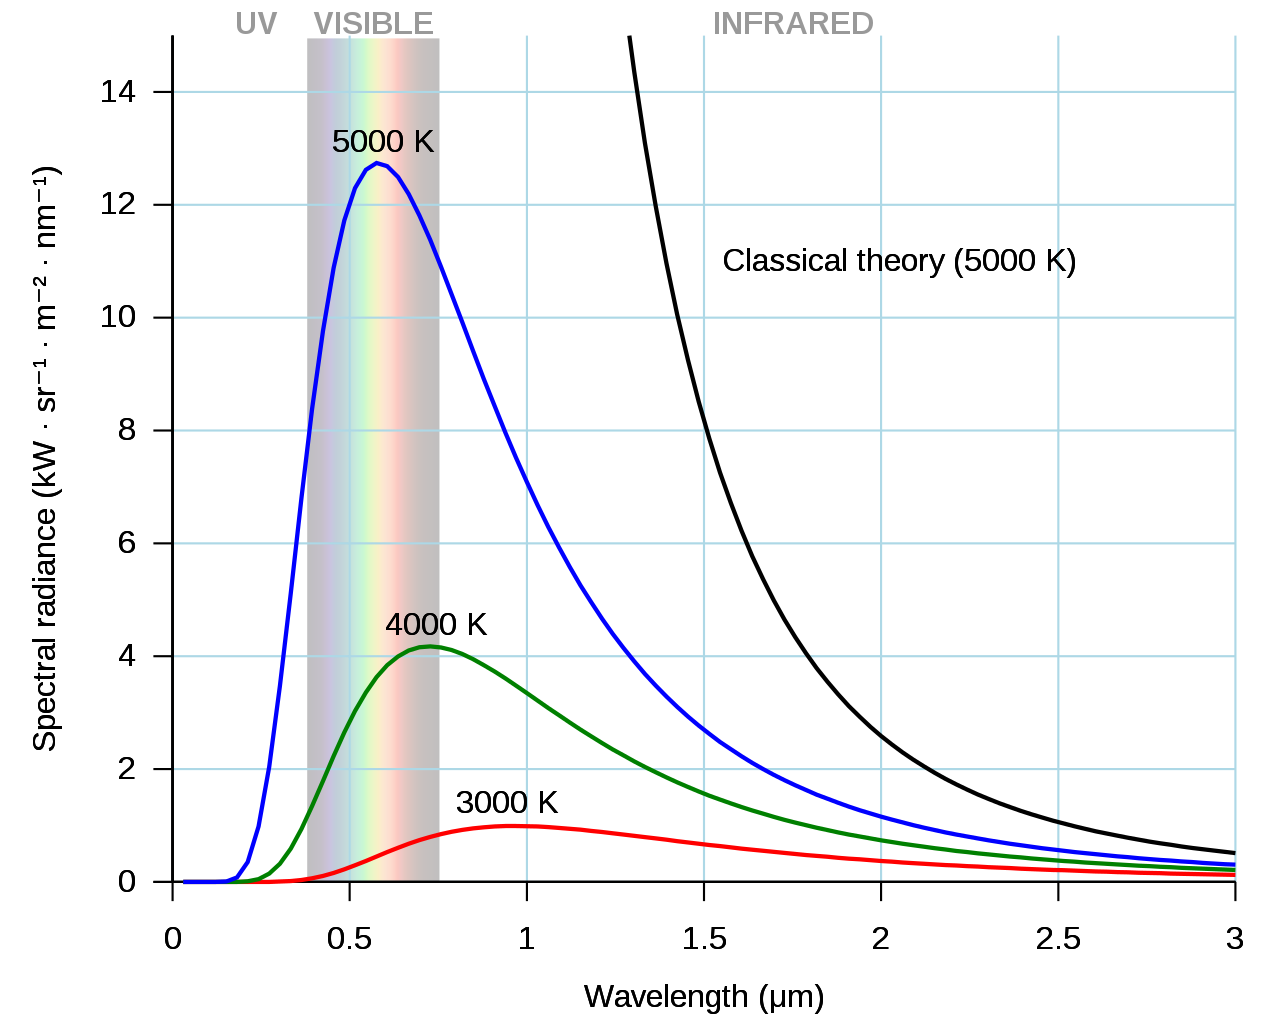
\includegraphics[width=\textwidth]{./images/1280px-Black_body.svg.png}
			\end{figure}
		\end{minipage}
		&
		\begin{minipage}[t]{.45\textwidth}	
			\begin{itemize}\scriptsize
				\item Kirchhoff’s law: 주어진 온도와 파장에서 방출과 흡수의 열역학적 관계\\
				- 복사 에너지를 잘 흡수하는 물체가 복사 에너지를 잘 방출한다.
				\item Planck’s law: 온도에 따른 흑체 복사의 강도 분포를 설명
				- 모든 물체는 항상 다양한 파장의 복사 에너지를 방출한다.
				$$
\begin{gathered}
					I(\nu, T)=\frac{2 h \nu^{3}}{c^{2}} \frac{1}{e^{\frac{h \nu}{k T}}-1} \\
					I^{\prime}(\lambda, T)=\frac{2 h c^{2}}{\lambda^{5}} \frac{1}{e^{\frac{h c}{\lambda k T}}-1}
				\end{gathered}
$$
			\end{itemize}
		\end{minipage}
	\end{tabular}
\end{frame}





\begin{frame}[t]{흑체 복사의 기본 법칙}
	\begin{tabular}{ll}
		\begin{minipage}[t]{.40\textwidth}
			\begin{figure}{}
				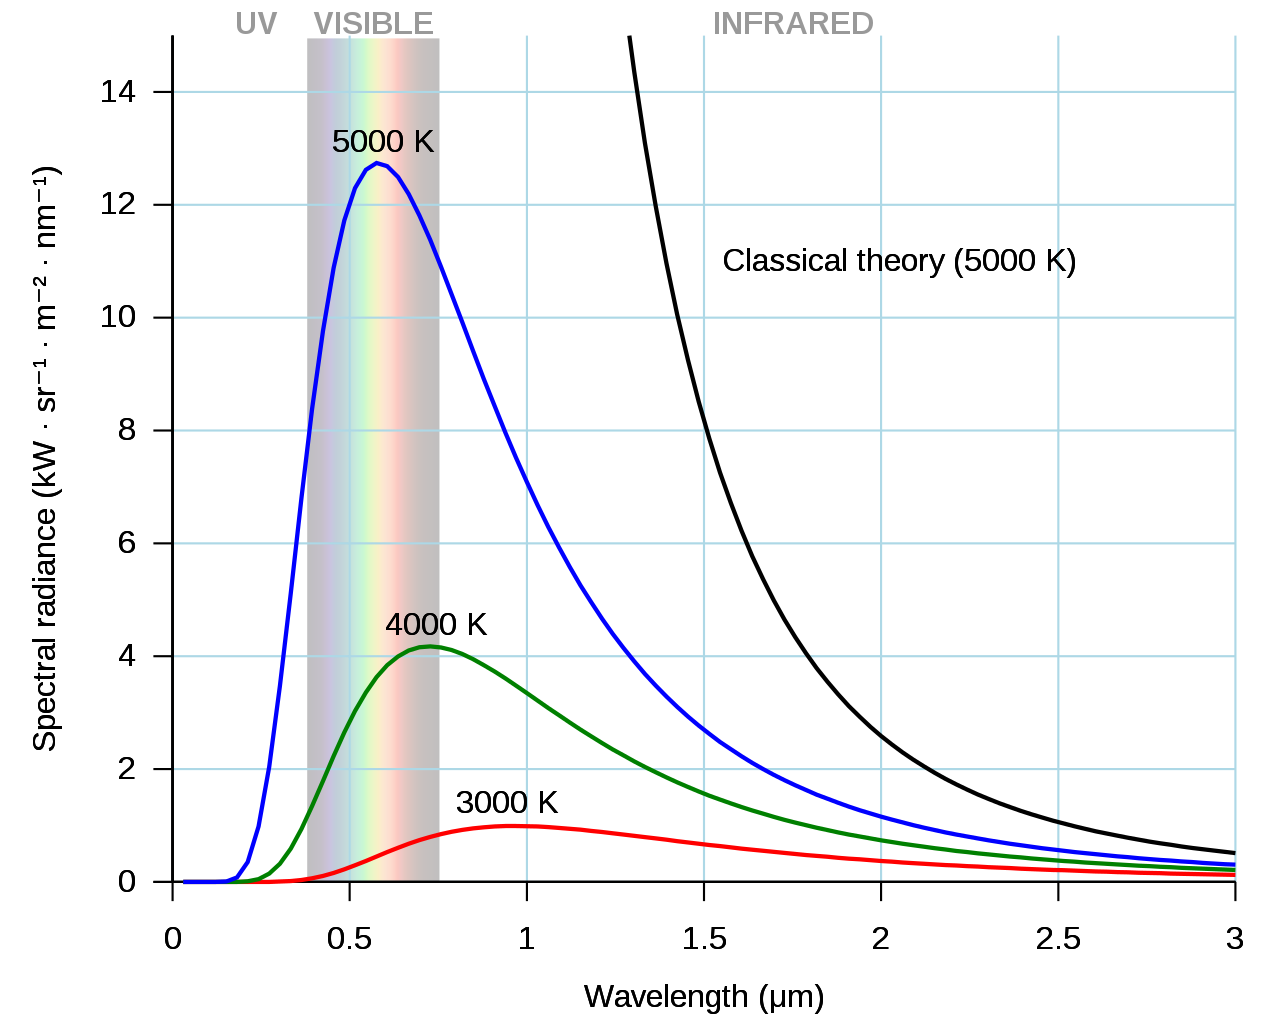
\includegraphics[width=\textwidth]{./images/1280px-Black_body.svg}
			\end{figure}
		\end{minipage}
		&
		\begin{minipage}[t]{.55\textwidth}	
			\begin{itemize}\scriptsize
				\item Stefan-Boltzmann’s law: 방출에너지의 시간변화율과 절대온도와의 관계 \\
				- 물체의 온도가 높을수록 단위 면적당 더 많은 에너지를 방출한다. \\
					$$ \begin{gathered}
						E=\sigma T^{4} \\
						\sigma=\frac{2 \pi^{5} k^{4}}{15 c^{2} h^{3}} = 5.670400 \times 10^{-8} \mathrm{~W} \mathrm{~m}^{-2} \mathrm{~K}^{-4}
					\end{gathered} $$
				\item Wien’s displacement law: 방출하는 최대 강도의 파장과 절대온도와의 관계\\
				- 물체의 온도가 높을수록 최대 복사의 파장은 짧아진다.	\\
					$$
\begin{gathered}
						\lambda_{\max } \cdot T=C \\
						C=2.898 \times 10^{-3} \mathrm{~m} \cdot \mathrm{K}
					\end{gathered}
$$
			\end{itemize}
		\end{minipage}
	\end{tabular}
\end{frame}




\begin{frame}[t]{태양 복사와 지구 복사}
	\begin{tabular}{ll}
		\begin{minipage}[t]{.950\textwidth}
			\begin{figure}{}
				\includegraphics[trim=50 50 30 460, clip, page=72, width=0.9\textwidth]{\bookfile} 
			\end{figure}
			\questionset{태양 복사와 지구 복사에서 자외선, 가시광선, 적외선 복사의 비중은 각각 어느 정도인가?}
			\solutionset{태양 복사:  7\%, 43\%, 49\%   지구 복사: 100\%}			
		\end{minipage}
		&
		\begin{minipage}[t]{.03\textwidth}	
			
		\end{minipage}
	\end{tabular}
\end{frame}



\begin{frame}[t]{자외선과 오존층}
	\begin{tabular}{ll}
		\begin{minipage}[t]{.5\textwidth}
			\begin{figure}{}
				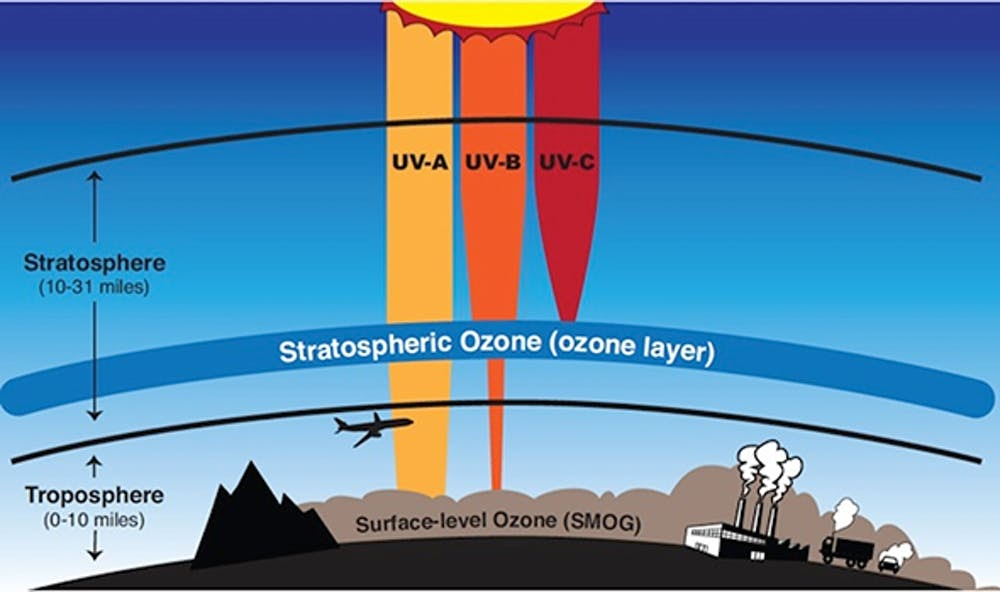
\includegraphics[width=\textwidth]{./images/file-20180418-163998-h02rtb} 
			\end{figure}
		\end{minipage}
		&
		\begin{minipage}[t]{.45\textwidth}
			\begin{figure}{}
				\includegraphics[trim=50 450 330 115, clip, page=74, width=\textwidth]{\bookfile} 
			\end{figure} 
		\end{minipage}
	\end{tabular}
	\begin{itemize}\scriptsize
		\item 자외선은 UVA($320 \sim 400 \rm{~nm}$), UVB($290 \sim 320 \rm{~nm}$), UVC($200 \sim 290 \rm{~nm}$)로 나뉨
		\item UVC는 지구의 표면에 도달하기 전 오존층에서 차단되고, UVA는 1년 내내 노출량이 같고, UVB는 여름에 특히 많아짐.
	\end{itemize}
\end{frame}



\begin{frame}[t]{자외선 지수}
	\begin{tabular}{ll}
		\begin{minipage}[t]{.45\textwidth}
			\begin{figure}{}
				\includegraphics[trim=330 455 55 108, clip, page=73, width=\textwidth]{\bookfile} 
			\end{figure}
			\begin{itemize}\scriptsize
				\item 과도한 자외선은 피부암, 백내장 등을 일으킴
			\end{itemize}
		\end{minipage}
		&
		\begin{minipage}[t]{.5\textwidth}
			\begin{figure}{}
				\includegraphics[trim=355 335 30 205, clip, page=74, width=\textwidth]{\bookfile} 
			\end{figure}	
			
		\end{minipage}
	\end{tabular}
\end{frame}









\section{입사 태양 복사는 어떻게 되는가}


\begin{frame}[t]{태양 복사 에너지의 분포}
	\begin{tabular}{ll}
		\begin{minipage}[t]{.650\textwidth}
			\begin{figure}{}
				\includegraphics[trim=40 40 70 460, clip, page=75, width=\textwidth]{\bookfile} 
			\end{figure}
		\end{minipage}
		&
		\begin{minipage}[t]{.3\textwidth}	
			\questionset{입사한 태양복사가 대기에 도달하면 어떤 일이 발생할 수 있는가?}
			\solutionset{투과 or 흡수 or 반사/산란 하게 하게 된다. \newline}
			
			\questionset{입사한 태양복사의 평균적인 지표, 대기, 구름에서의 분포를 설명하시오}
			\solutionset{지표 흡수: 50\%, \\
				구름, 대기 흡수: 20\%, \\
				구름 반사: 20\%, \\
				대기 후방 산란: 5\%, \\
				지표, 해수면 반사: 5\%}
		\end{minipage}
	\end{tabular}
\end{frame}






\begin{frame}[t]{반사와 산란}
	\begin{tabular}{ll}
		\begin{minipage}[t]{.45\textwidth}
			\begin{figure}{}
				\includegraphics[trim=50 450 335 60, clip, page=76, width=\textwidth]{\bookfile} 
			\end{figure}
		\end{minipage}
		&
		\begin{minipage}[t]{.50\textwidth}	
			\begin{figure}{}
				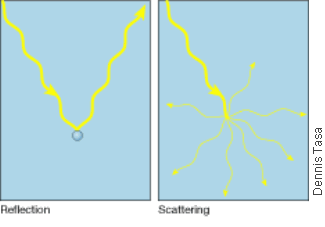
\includegraphics[width=0.7\textwidth]{./images/XxRaPyyhQGGJWvGpPhUk_Module7-012}
			\end{figure}
			\begin{itemize}\scriptsize
				\item 반사는 빛이 물체의 표면과 만나는 각도와 같은 각도에서 같은 강도로 되돌아 가는 것
				\item 산란은 빛이 약화되어 다른 방향으로 무수히 흩어지는 것
			\end{itemize}	
		\end{minipage}
	\end{tabular}
\end{frame}






\begin{frame}[t]{레일리 산란(Rayleigh scattering)}
	\begin{tabular}{ll}
		\begin{minipage}[t]{.55\textwidth}
			\begin{figure}{}
				\includegraphics[trim=50 535 230 60, clip, page=77, width=\textwidth]{\bookfile} 
			\end{figure}
		\end{minipage}
		&
		\begin{minipage}[t]{.4\textwidth}	
			\begin{itemize}\scriptsize
				\item 산란하는 입자의 크기가 파장보다 훨씬 작은 경우
				\item 산란 강도는 파장의 4제곱에 반비례\\
				$${\displaystyle I \propto	\frac{1}{\lambda^{4}}}$$
				\item 우리 대기의 구성 입자(분자)에 의한 산란이 여기에 해당
			\end{itemize}
		\end{minipage}
			
		\questionset {맑은날 하늘이 파랗게 보이는 이유를 설명하시오.}
		\solutionset{짧은 파장이 더 쉽게 산란되므로 우리 눈에 산란광이 도달하여 하늘이 푸르게 보인다. \newline}

		\questionset{일출이나 일몰 시 하늘이 붉게 보이는 이유를 설명하시오.}
		\solutionset{대기의 광학적 두께가 두꺼워지는 일출, 일몰 시에는 단파장 영역의 빛이 대부분 산란되어 장파장 영역의 빛이 주로 도달하여 하늘이 붉게 보임(노을의 원리)}
	\end{tabular}
\end{frame}





\begin{frame}[t]{미 산란(Mie scattering)}
	\begin{tabular}{ll}
		\begin{minipage}[t]{.600\textwidth}
			\begin{figure}{}
				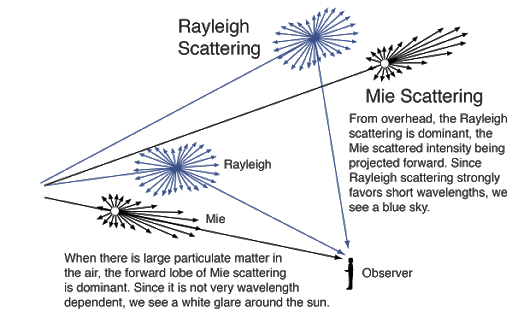
\includegraphics[width=\textwidth]{./images/scattering} 
			\end{figure}
		\end{minipage}
		&
		\begin{minipage}[t]{.350\textwidth}	
			\begin{itemize}\scriptsize
				\item 먼지와 같은 에어로졸과 빗방울 처럼 산란하는 입자의 크기가 더 커진 경우
				\item 입자 위의 한 점으로부터 산란된 빛과 다른 점으로부터 산란된 빛의 위상이 어긋나 간섭이 발생하며 산란광의 분포도 레일리 산란과 다름
				\item 산란 강도는 파장과 무관함
				\end{itemize}
			
				\questionset {구름이나 안개, 스모그 현상 시 하얗게 보이는 이유는?}
				\solutionset{물방울, 먼지는 빛의 파장보다 크기가 커서 Mie 산란을 일으켜 모든 파장에서 고르게 빛을 산란시키므로}
		\end{minipage}
	\end{tabular}
\end{frame}






\begin{frame}[t]{반사율(albedo)}
	\begin{tabular}{ll}
		\begin{minipage}[t]{.50\textwidth}
			\begin{figure}{}
				\includegraphics[trim=350 50 45 440, clip, page=76, width=\textwidth]{\bookfile} 
			\end{figure}
		\end{minipage}
		&
		\begin{minipage}[t]{.450\textwidth}	
			\begin{itemize}\scriptsize
				\item 지표에 의해 반사된 복사 에너지의 비율
				\item 특정 파장에 대해 정의하지 않고 전 파장영역에 걸친 평균값으로 정의
				\item 입사광의 각도 분포나 대기의 투과율, 지표 성질에 의해서 변화할 수 있는 값
			\end{itemize}
			\questionset {어떤 곳이 알베도가 높은가?}
			\solutionset{눈, 두꺼운 구름, 수면 등 \newline}
			
			\questionset {구름이 알베도에 미치는 영향은 어떨까?}
			\solutionset{낮고 두꺼운 구름은 태양 복사를 반사하여 알베도를 높여 냉각 효과를 일으키고, 높고 얇은 구름은 대부분의 태양 복사가 반사 없이 지표에 도달, 지구 복사는 흡수하여 가열 효과을 일으킨다. 종합적으로는 냉각 효과가 일어난다.}
		\end{minipage}
	\end{tabular}
\end{frame}





\section{대기 중 기체의 역할}


\begin{frame}[t]{태양 복사와 지구 복사}
	\begin{tabular}{ll}
		\begin{minipage}[t]{.55\textwidth}
			\begin{figure}{}
				\includegraphics[trim=270 330 50 230, clip, page=79, width=\textwidth]{\bookfile} 
			\end{figure}
		\end{minipage}
		&
		\begin{minipage}[t]{.40\textwidth}	
			\begin{itemize}
				\item 태양 복사는 자외선, 가시광선, 적외선, 단파복사($2.5 \rm{~\mu m}$ 보다 짧은 파장)
				\item 지구 복사의 대부분은 적외선, 장파복사($2.5 \sim 30 \rm{~\mu m}$)
			\end{itemize}	
			\questionset{태양($5800\rm{~K}$)과 지구($288 \rm{~K}$)의 $\lambda _{\textrm{max}}$ 를 계산해 보자.}
			\solutionset{$$ \begin{gathered}
					\lambda_{\max } \cdot T=C \\
					C=2.898 \times 10^{-3} \mathrm{~m} \cdot \mathrm{K}
				\end{gathered} $$
			태양 : 약 $0.5\rm{~\mu m}$, 지구 : 약 $10\rm{~\mu m}$}
		\end{minipage}
	\end{tabular}
\end{frame}






\begin{frame}[t]{대기를 가열하기}
	\begin{tabular}{ll}
		\begin{minipage}[t]{.350\textwidth}
			\begin{figure}{}
				\includegraphics[trim=270 40 50 230, clip, page=79, width=\textwidth]{\bookfile} 
			\end{figure}
		\end{minipage}
		&
		\begin{minipage}[t]{.60\textwidth}	
			\begin{itemize}
				\item $0.3 \sim 0.7\rm{~\mu m}$ 파장의 가시광에 대해 어떤 기체도 효과적 흡수체가 아니므로 대기는 입사하는 태양 복사에 대해 거의 투명함.
				\item 반면, 장파장인 지구 복사에 대해 상대적으로 효과적인 흡수체이며, 대기는 지구 복사의 약 60\% 정도를 흡수함.(불투명함)
				\item 태양 복사에 대한 효과적인 흡수체는 수증기, 산소, 오존이며, 
				\item 지구 복사에 대한 효과적인 흡수체는 수증기, 이산화 탄소임.
			\end{itemize}	
		\end{minipage}
	\end{tabular}
\end{frame}




\begin{frame}[t]{복사 에너지의 선택적 흡수}
	\begin{tabular}{ll}
		\begin{minipage}[t]{.45\textwidth}
			\begin{figure}{}
				\includegraphics[trim=270 40 50 410, clip, page=79, width=\textwidth]{\bookfile} 
			\end{figure}
		\end{minipage}
		&
		\begin{minipage}[t]{.50\textwidth}	
			\questionset{’대기의 창’이란 무엇이며, 어떤 경우에 닫히기도 하는가?}
			\solutionset{지구 복사 중 $8 \sim 12\rm{~\mu m}$ 파장 대역의 복사는 대기에 의해 거의 흡수되지 않는데, 이를 대기의 창이라고 부른다.\\			
			작은 물방울로 된 구름은 장파 복사를 잘 흡수하며, 이 에너지의 상당 부분을 지표로 방출한다. 따라서 대기의 창을 닫는 역할을 하며, 지표가 냉각되는 속도를 느리게 한다.\newline}
			
			\questionset{기상 위성의 수증기 채널로 사용하기 적합한 파장대는 얼마인가?}
			\solutionset{수증기에 의해서는 흡수되지만 다른 기체에 의해서는 거의 흡수되지 않는 $6 \sim 7 \rm{~\mu m}$ 영역이 수증기를 검출하는데 유용하다.\newline}
			
			\questionset{기상 위성의 적외선 채널은 두 개의 파장대는 얼마이며 이를 구분해주는 기체는 어떤 성분인가?}
			\solutionset{중심파장이 각각 IR1은 $10.8 \rm{~\mu m}$,  IR2는 $12.0 \rm{~\mu m}$ 
			이며, 이 둘의 사이는 산소와 오존에 의해 나누어진다.\newline}
			
		\end{minipage}
	\end{tabular}
\end{frame}








\begin{frame}[t]{복사평형 온도}
	\begin{tabular}{ll}
		\begin{minipage}[t]{.50\textwidth}
			\begin{figure}{}
				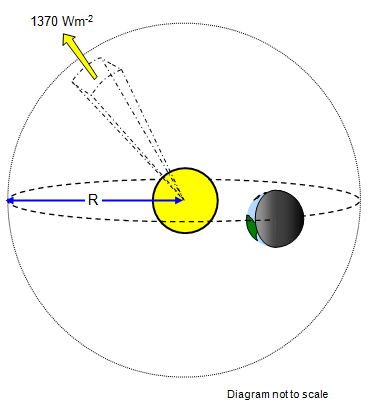
\includegraphics[width=0.5\textwidth]{./images/solar_constants} 
			\end{figure}
		\begin{figure}{}
			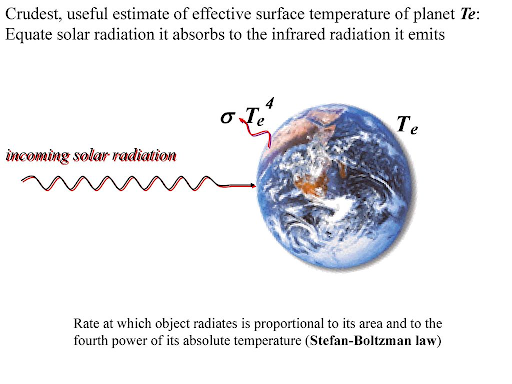
\includegraphics[trim=0 110 60 85, clip, width=\textwidth]{./images/earth_temp} 
		\end{figure}
		\end{minipage}
			&
		\begin{minipage}[t]{.450\textwidth}
		\questionset{각 행성에서의 태양 상수는 어떻게 되는가? (단, 지구의 태양 상수는 $S_{0}$, 태양- 지구 사이의 평균 거리는 $r_{0}$, 태양 행성 사이의 평균 거리는 $r_{p}$이다.)}
		\solutionset{$$ S_{p}=S_{0}\left(\dfrac{r_{0}}{r_{p}}\right)^{2}$$ \newline}

		\questionset{그림을 참고하여 행성의 복사평형 온도($T_e$)를 식으로 나타내면? (단, 행성의 태양 상수는 $S_{p}$, 행성의 반지름은 $R_{p}$, 반사율 $A$라 하고, 대기의 온실 효과는 고려하지 않는다.)}
		\solutionset{$$
\begin{gathered}
				\pi R_{p}^{2}(1-A) S_{p}=4 \pi R_{p}^{2} \sigma T_{e}^{4} \\
				T_{e}=\left(\frac{1-A}{4 \sigma} S_{p}\right)^{\frac{1}{4}}
			\end{gathered}
$$ }
		\end{minipage}
		\end{tabular}
\end{frame}






\begin{frame}[t]{복사평형 온도}
	\begin{tabular}{ll}
		\begin{minipage}[t]{.20\textwidth}
			\begin{figure}{}
				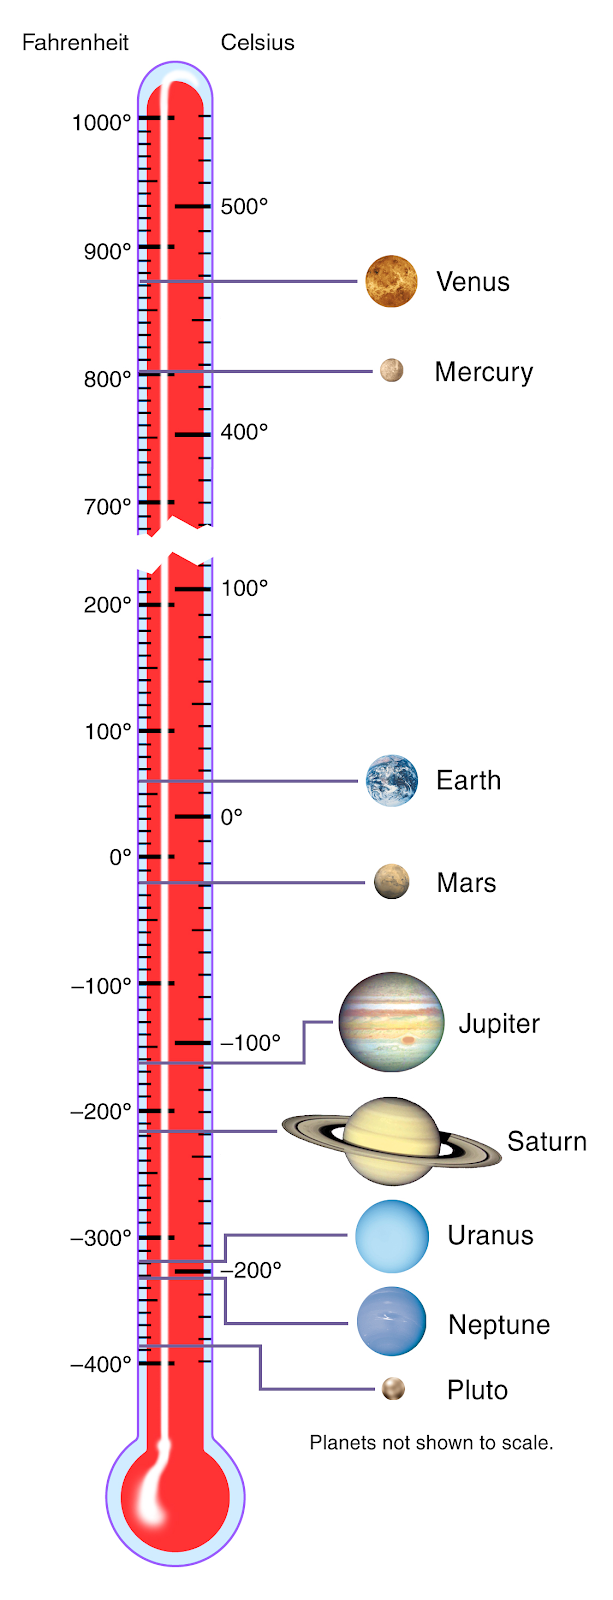
\includegraphics[width=\textwidth]{./images/temp_of_planets} 
			\end{figure}
		\end{minipage}
		&
		\begin{minipage}[t]{.750\textwidth}			
			\questionset{태양계 행성들의 복사평형 온도를 계산해 보자.}
			\solutionset{실험 시간에 Python으로}
		\end{minipage}
	\end{tabular}
\end{frame}




\begin{frame}[t]{복사평형}
	\begin{tabular}{ll}
		\begin{minipage}[t]{.70\textwidth}
			\begin{figure}{}
				\includegraphics[trim=30 402 30 62, clip, page=81, width=\textwidth]{\bookfile} 
			\end{figure}
			\begin{itemize}\scriptsize
			\item 복사평형(흡수E = 방출E): 행성(위성)들은 태양으로부터 받은 복사에너지와 같은 양의 에너지를 다시 우주 공간으로 방출하여 장기적 관점에서 온도는 일정하게 유지된다.
			\end{itemize}
		\end{minipage}
		&
		\begin{minipage}[t]{.25\textwidth}	
			\questionset{지구와 달의 복사평형 온도는 $255 \rm{~K}$로 같은데, 지구의 평균 온도는 $288 \rm{~K}$인 이유는 무엇인가?}
			\solutionset{지구와 달은 태양과의 평균 거리가 비슷하므로 태양 상수가 같아 복사평형 온도는 $288 \rm{~K}$로 같지만, 지구는 온실효과로 약 $33 \rm{~K}$ 가량 기온이 높게 나타난다.}

		\end{minipage}
	\end{tabular}
\end{frame}





\section{지구의 에너지 수지}




\begin{frame}[t]{에너지 수지}
	\begin{tabular}{ll}
		\begin{minipage}[t]{.80\textwidth}
			\begin{figure}{}
				\includegraphics[trim=55 380 50 60, clip, page=82, width=\textwidth]{\bookfile} 
			\end{figure}
		\end{minipage}
		&
		\begin{minipage}[t]{.150\textwidth}	
			\questionset{지구의 연간 에너지 수지 값을 설명하시오.}
			\solutionset{우주공간, 대기, 지표로 구분하여
				각각 흡수하는 에너지(+)와 방출하는 에너지(-)의 합이 0이 되는지 확인.}
		\end{minipage}
	\end{tabular}
\end{frame}





\begin{frame}[t]{위도별 열수지}
	\begin{tabular}{ll}
		\begin{minipage}[t]{.40\textwidth}
			\begin{figure}{}
				\includegraphics[trim=60 370 360 60, clip, page=83, width=0.8\textwidth]{\bookfile} 
			\end{figure}
		\end{minipage}
		&
		\begin{minipage}[t]{.550\textwidth}	
			\questionset{그림과 같이 적도 지방과 극 지방 사이의 열 불균형이 나타나는 이유와 열 불균형으로 인해 나타나는 현상은?}
			\solutionset{적도 지방은 일반적으로 태양의 고도가 높아 입사하는 복사 에너지가 방출되는 복사보다 많지만, 극 지방은 반대가 되기 때문에 해류와 바람을 통해 적도 지방의 누적된 열이 극지방으로 이동한다.}
		\end{minipage}
	\end{tabular}
\end{frame}

